\chapter{Metodolog\'ia Experimental y Configuraci\'on de la Simulaci\'on}
\label{chap:metodologia}

Este cap\'itulo detalla el dise\~no metodol\'ogico implementado para la simulaci\'on termodin\'amica y econ\'omica de los sistemas de enfriamiento de alta densidad ($100\text{ kW}$ por rack), as\'i como la arquitectura del pipeline de datos e integraci\'on con la nube de Google Cloud Platform (GCP).

\section{Arquitectura del Simulador (Python)}
El modelamiento del comportamiento t\'ermico y de costos operativos se program\'o en el entorno local utilizando Python 3.11, estructurado en dos scripts principales:
\begin{enumerate}
    \item \textbf{\texttt{simulador\_ia\_100kw.py}}: Contiene la l\'ogica f\'isica para calcular el PUE din\'amico hora a hora.
    \item \textbf{\texttt{termo\_economia\_global.py}}: Ejecuta las simulaciones multianuales a gran escala, integrando los costos de electricidad industrial y fuentes de tarifas reales para cada ubicaci\'on geogr\'afica.
\end{enumerate}

La simulaci\'on se configur\'o con par\'ametros constantes representativos de la demanda de superc\'omputo de Inteligencia Artificial para el a\~no 2026:
\begin{itemize}
    \item Carga T\'ermica de TI ($P_{IT}$): $100\text{ kW}$ constantes ($24/7/365$).
    \item Rango de Operaci\'on del Procesador: Temperatura de uni\'on m\'axima permitida en el silicio ($T_{j,max}$) de $75^\circ\text{C}$ para evitar estrangulamiento t\'ermico.
    \item Flujo Volum\'etrico de Fluidos Diel\'ectricos: Configurado en $\dot{V}_{\text{bifasico}} = 0,6\text{ L/s}$ para ebullici\'on saturada (ej. 3M Novec 7100), logrando una reducci\'on volum\'etrica de $9.200$ veces en comparaci\'on con el caudal de aire requerido ($5.520\text{ L/s}$) para disipar la misma carga.
\end{itemize}

\section{Modelamiento del PUE Din\'amico}
El c\'alculo del PUE din\'amico de enfriamiento se rige por la relaci\'on entre la temperatura del aire exterior ($T_{ext}$) y la temperatura cr\'itica de transici\'on ($T_{cr}$) definida para cada tecnolog\'ia:
\begin{itemize}
    \item \textbf{Rear Door Heat Exchanger (RDHx) Baseline:} $T_{cr} = 10,0^\circ\text{C}$, $T_{max} = 40,0^\circ\text{C}$; $PUE_{fc} = 1,15$, $PUE_{base} = 1,50$.
    \item \textbf{Termosif\'on Direct-to-Chip (D2C) Bif\'asico:} $T_{cr} = 25,0^\circ\text{C}$, $T_{max} = 40,0^\circ\text{C}$; $PUE_{fc} = 1,05$, $PUE_{base} = 1,20$.
    \item \textbf{Inmersi\'on L\'iquida Bif\'asica:} $T_{cr} = 35,0^\circ\text{C}$, $T_{max} = 45,0^\circ\text{C}$; $PUE_{fc} = 1,02$, $PUE_{base} = 1,10$.
\end{itemize}

\section{Descripci\'on y Esquemas de los Sistemas de Enfriamiento}
En esta secci\'on se detalla la configuraci\'on f\'isica y el principio termodin\'amico de funcionamiento de las tres tecnolog\'ias evaluadas, representadas vectorialmente mediante diagramas en TikZ.

\subsection{Rear Door Heat Exchanger (RDHx)}
El sistema RDHx (Fig.~\ref{fig:rdhx_diagram}) es una tecnolog\'ia h\'ibrida de aire-l\'iquido. En lugar de enfriar el aire de la sala, se acopla un intercambiador de calor de tubos aleteados directamente en la puerta trasera del rack. El aire caliente sale de los servidores empujado por los ventiladores del chasis, atraviesa las bobinas de cobre del RDHx donde rechaza el calor hacia un circuito secundario de agua a temperatura templada, y sale de la puerta a temperatura neutral.

\begin{figure}[htbp]
\centering
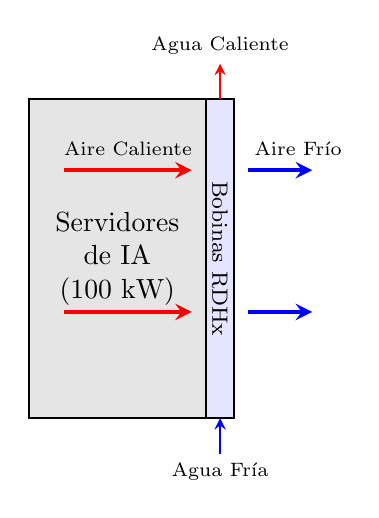
\begin{tikzpicture}[scale=0.9, >=stealth]
    % Draw Rack cabinet
    \draw[thick, fill=gray!20] (0,0) rectangle (2.5,4.5);
    \node at (1.25,2.25) [align=center] {Servidores\\de IA\\(100 kW)};
    
    % Draw Rear Door (RDHx)
    \draw[thick, fill=blue!10] (2.5,0) rectangle (2.9,4.5);
    \node[rotate=-90] at (2.7,2.25) {\footnotesize Bobinas RDHx};
    
    % Draw airflow arrows
    \draw[->, red, ultra thick] (0.5,3.5) -- (2.3,3.5);
    \draw[->, red, ultra thick] (0.5,1.5) -- (2.3,1.5);
    \node at (1.4,3.8) {\scriptsize Aire Caliente};
    
    \draw[->, blue, ultra thick] (3.1,3.5) -- (4.0,3.5);
    \draw[->, blue, ultra thick] (3.1,1.5) -- (4.0,1.5);
    \node at (3.8,3.8) {\scriptsize Aire Fr\'io};
    
    % Draw water loop pipes
    \draw[blue, thick, ->] (2.7, -0.5) -- (2.7, 0);
    \draw[red, thick, ->] (2.7, 4.5) -- (2.7, 5.0);
    \node[below] at (2.7,-0.5) {\scriptsize Agua Fr\'ia};
    \node[above] at (2.7,5.0) {\scriptsize Agua Caliente};
\end{tikzpicture}
\caption{Diagrama esquem\'atico del intercambiador de calor en la puerta trasera (RDHx).}
\label{fig:rdhx_diagram}
\end{figure}

\subsection{Termosif\'on Direct-to-Chip (D2C) Bif\'asico}
El termosif\'on D2C bif\'asico (Fig.~\ref{fig:d2c_diagram}) utiliza un circuito cerrado sin bombeo mec\'anico activo, aprovechando el cambio de fase de un fluido diel\'ectrico. El refrigerante l\'iquido ingresa a las placas fr\'ias evaporadoras acopladas sobre las CPU/GPU. La alta densidad de calor hace hervir el fluido a temperatura constante. El vapor generado, de baja densidad, asciende por el elevador hacia el condensador superior, donde condensa al transferir calor al lazo secundario, retornando l\'iquido por gravedad.

\begin{figure}[htbp]
\centering
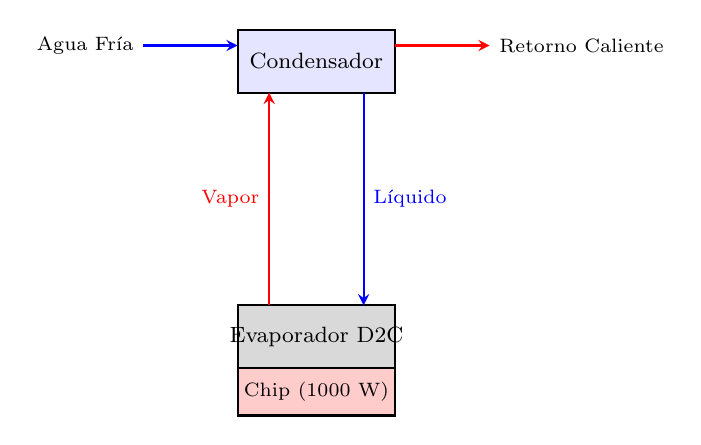
\begin{tikzpicture}[scale=1.0, >=stealth]
    % Evaporator
    \draw[thick, fill=gray!30] (0,0) rectangle (2,0.8);
    \node at (1,0.4) {\footnotesize Evaporador D2C};
    \draw[thick, fill=red!20] (0,-0.6) rectangle (2,0);
    \node at (1,-0.3) {\scriptsize Chip (1000 W)};

    % Condenser
    \draw[thick, fill=blue!10] (0,3.5) rectangle (2,4.3);
    \node at (1,3.9) {\footnotesize Condensador};

    % Vapor line (Ascend)
    \draw[->, red, thick] (0.4, 0.8) -- (0.4, 3.5);
    \node[left, red] at (0.4, 2.15) {\scriptsize Vapor};

    % Liquid return line (Gravity drain)
    \draw[<-, blue, thick] (1.6, 0.8) -- (1.6, 3.5);
    \node[right, blue] at (1.6, 2.15) {\scriptsize L\'iquido};

    % Facility water loop on condenser
    \draw[blue, thick, ->] (-1.2, 4.1) -- (0, 4.1);
    \draw[red, thick, ->] (2, 4.1) -- (3.2, 4.1);
    \node[left] at (-1.2, 4.1) {\scriptsize Agua Fr\'ia};
    \node[right] at (3.2, 4.1) {\scriptsize Retorno Caliente};
\end{tikzpicture}
\caption{Diagrama esquem\'atico del termosif\'on Direct-to-Chip (D2C) bif\'asico.}
\label{fig:d2c_diagram}
\end{figure}

\subsection{Inmersi\'on L\'iquida Bif\'asica}
En la inmersi\'on bif\'asica (Fig.~\ref{fig:immersion_diagram}), los servidores de IA se sumergen completamente en un tanque herm\'etico lleno de refrigerante diel\'ectrico con bajo punto de ebullici\'on. El fluido hierve en contacto directo con el silicio caliente, formando burbujas de vapor que ascienden a la superficie del l\'iquido. En la c\'upula sellada, el vapor choca contra un serpent\'in condensador refrigerado por agua de torre, volviendo al estado l\'iquido y goteando de vuelta al tanque de forma continua.

\begin{figure}[htbp]
\centering
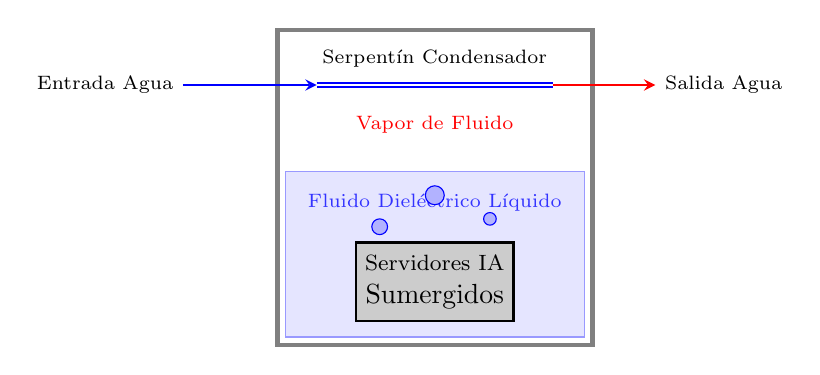
\begin{tikzpicture}[scale=1.0, >=stealth]
    % Tank walls
    \draw[ultra thick, gray] (0,0) -- (0,4) -- (4,4) -- (4,0) -- cycle;
    
    % Liquid level
    \draw[blue!40, fill=blue!10] (0.1,0.1) rectangle (3.9,2.2);
    \node[blue!80] at (2.0,1.8) {\scriptsize Fluido Diel\'ectrico L\'iquido};
    
    % Submerged server
    \draw[thick, fill=gray!40] (1.0,0.3) rectangle (3.0,1.3);
    \node at (2.0,0.8) [align=center] {\footnotesize Servidores IA\\Sumergidos};
    
    % Bubbles / Vapor rising
    \draw[fill=blue!30, draw=blue] (1.3,1.5) circle (0.1);
    \draw[fill=blue!30, draw=blue] (2.7,1.6) circle (0.08);
    \draw[fill=blue!30, draw=blue] (2.0,1.9) circle (0.12);
    \node[red] at (2.0,2.8) {\scriptsize Vapor de Fluido};
    
    % Condenser coil at the top
    \draw[thick, double, blue] (0.5,3.3) -- (3.5,3.3);
    \node[above] at (2.0,3.4) {\scriptsize Serpent\'in Condensador};
    
    % Facility water pipes
    \draw[blue, thick, ->] (-1.2, 3.3) -- (0.5, 3.3);
    \draw[red, thick, ->] (3.5, 3.3) -- (4.8, 3.3);
    \node[left] at (-1.2, 3.3) {\scriptsize Entrada Agua};
    \node[right] at (4.8, 3.3) {\scriptsize Salida Agua};
\end{tikzpicture}
\caption{Diagrama esquem\'atico del sistema de inmersi\'on l\'iquida bif\'asica.}
\label{fig:immersion_diagram}
\end{figure}


\section{Pipeline de Datos e Ingesta en GCP}
Para procesar de forma masiva los datos meteorol\'ogicos de 39 localidades geogr\'aficas ($26.280\text{ horas}$ por ubicaci\'on, totalizando $1.025.856$ registros de temperatura), se dise\~n\'o un flujo de trabajo ETL (Extract, Translate, Load) automatizado:
\begin{enumerate}
    \item \textbf{Descarga:} Obtenci\'on de las temperaturas hist\'oricas horarias (2023--2025) mediante la API de Open-Meteo.
    \item \textbf{Estructuraci\'on:} Conversi\'on de columnas a snake\_case y formateo del tiempo a Timestamp mediante pandas en \texttt{data\_fetcher\_global.py}.
    \item \textbf{Carga inicial:} Ingesta de datos a Google BigQuery mediante \texttt{upload\_data\_centers\_bq.py} en el dataset \texttt{data\_center\_research} del proyecto \texttt{project-5ca89b0c-e364-4245-a61}.
    \item \textbf{Ingesta incremental:} Script \texttt{daily\_weather\_etl.py} que consulta de manera diaria el clima del d\'ia anterior de las 6 ciudades clave y lo sube a la tabla.
\end{enumerate}

Para asegurar la idempotencia del ETL en el Sandbox de GCP (que restringe el uso de DML \texttt{DELETE}), el script realiza una comprobaci\'on \texttt{SELECT COUNT(1)} de la fecha del d\'ia. Si el conteo es mayor que cero, salta la inserci\'on previniendo registros duplicados.

\section{Esquema de Base de Datos en BigQuery}
Los datos se estructuraron bajo dos tablas en BigQuery:
\begin{itemize}
    \item \textbf{\texttt{climate\_data\_global}:} Almacena las variables de clima hist\'orico e incremental: \texttt{location} (STRING), \texttt{region} (STRING), \texttt{latitude} (FLOAT), \texttt{longitude} (FLOAT), \texttt{time} (TIMESTAMP) y \texttt{temperature\_c} (FLOAT).
    \item \textbf{\texttt{analisis\_termoeconomico\_global}:} Almacena los resultados de costos calculados trienales: \texttt{region} (STRING), \texttt{localidad} (STRING), \texttt{precio\_usd\_kwh} (FLOAT), \texttt{fuente\_tarifa} (STRING), \texttt{url\_fuente} (STRING), \texttt{sistema\_enfriamiento} (STRING), \texttt{horas\_totales} (INTEGER), \texttt{free\_cooling\_hours} (INTEGER), \texttt{fch\_pct} (FLOAT), \texttt{energia\_total\_kwh} (FLOAT) y \texttt{opex\_3\_anios\_usd} (FLOAT).
\end{itemize}

\section{Entrenamiento del Modelo ARIMA\_PLUS en BigQuery ML}
El entrenamiento predictivo se configur\'o utilizando BigQuery ML mediante el script \texttt{train\_cooling\_model.py}. Esto permite entrenar de forma paralela 6 modelos individuales utilizando la opci\'on \texttt{time\_series\_id\_col='location'}. El modelo de series de tiempo resultante, \texttt{cooling\_forecast\_model}, se registra autom\'aticamente en el Vertex AI Model Registry de GCP para permitir su posterior consumo u operaci\'on automatizada en la nube.
